\section{Experimental Results}
\label{sec:experiments}

We evaluate Kimodo-Policy's control performance and deployment feasibility through single- and multi-task experiments on HumanoidArena (Sec.~\ref{sec:exp_simulation}), manipulation tasks on SIMPLE (Sec.~\ref{sec:exp_simple}), and real-world deployment (Sec.~\ref{sec:exp_real}). We then examine T2M backbone quality (Sec.~\ref{sec:exp_t2m}), data and model scaling (Sec.~\ref{sec:exp_scaling}), and key design choices through ablations (Sec.~\ref{sec:exp_ablation}). Details of the datasets, training protocols, and evaluation environments are provided in Appendix~\ref{sec:experimental_setup}.

\subsection{Evaluation on the HumanoidArena Benchmark}
\label{sec:exp_simulation}

HumanoidArena~\cite{humanoidarena} comprises seven language-conditioned humanoid tasks spanning human--object interaction (HOI) and human--scene interaction (HSI), as illustrated in Fig.~\ref{fig:humanoidarena}. We evaluate Kimodo-Policy in two settings: independent fine-tuning on each task and joint training across multiple SONIC tasks, covering single-task capability and the more challenging multi-task setting.

\begin{figure}[H]
  \centering
  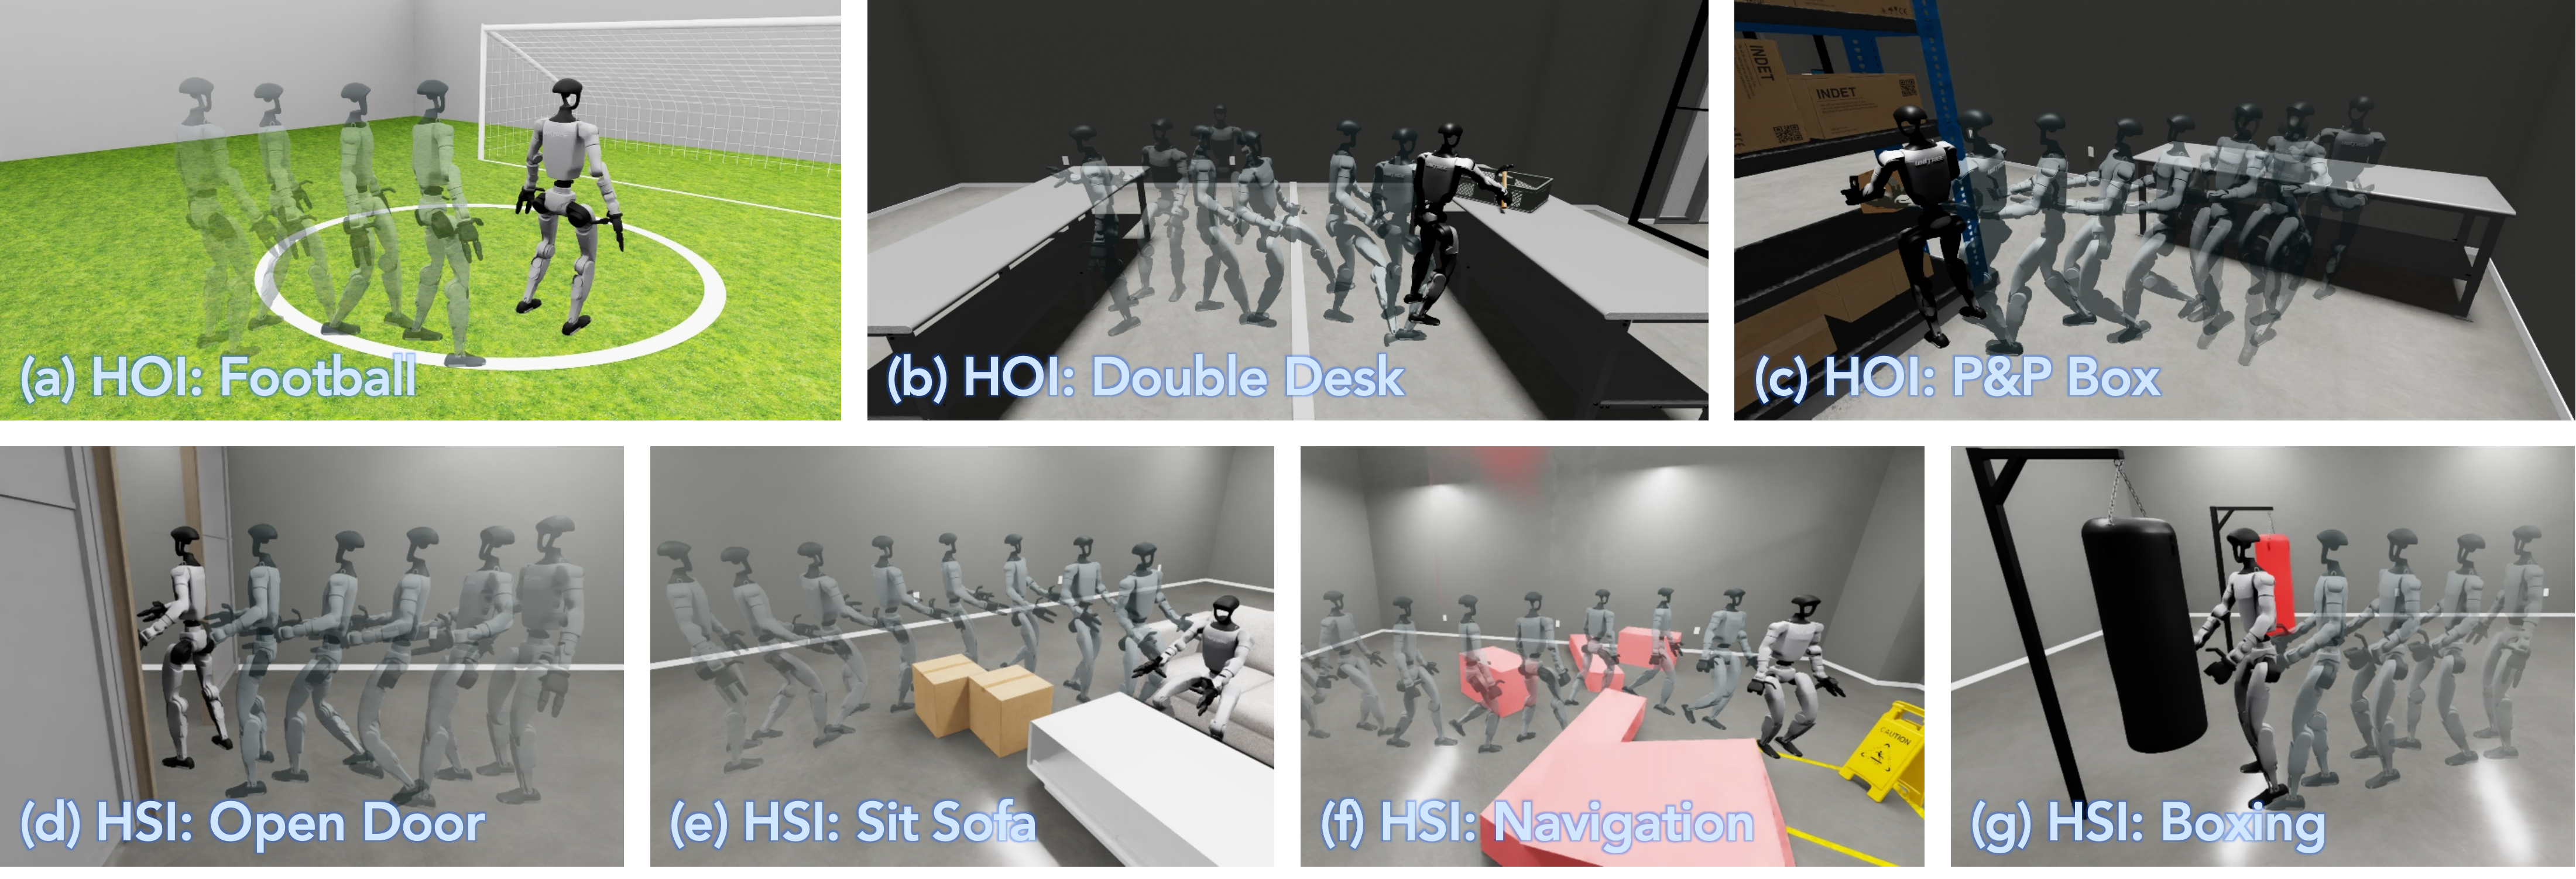
\includegraphics[width=\textwidth]{image/arena.png}
  \caption{\textbf{Visualization of the Seven HumanoidArena Tasks.} The benchmark includes Football, DoubleDesk, P\&Pbox, OpenDoor, SitSofa, Boxing, and VisNavi, covering language-conditioned humanoid behavior across human--object and human--scene interaction with coordinated locomotion, balance, and manipulation.}
  \label{fig:humanoidarena}
\end{figure}

\textbf{Single-task results.} We fine-tune a separate policy for each HumanoidArena task and compare two initialization strategies: Kimodo-Policy is fine-tuned directly on the task data, whereas Kimodo-Policy$^{*}$ initializes its ControlNet and hand head from our 419-hour VLA policy-pretraining stage. To ensure a fair comparison with the reported baselines, RTC is disabled when evaluating both variants. Under this setting, Kimodo-Policy achieves the highest overall success rate (SR) at 69.51\%, exceeding the strongest baseline, DP~\cite{chi2023diffusionpolicy} (60.0\%), by 9.51 percentage points. It also attains the lowest average fall rate (AFR; 4.29\%, tied with Kimodo-Policy$^{*}$) and the highest average SR on human--scene interaction (HSI; 84.58\%). The VLA-pretrained variant achieves 67.14\% overall SR and an 84.17\% HSI average, with the highest task-level SRs on OpenDoor (93.3\%) and VisNavi (76.7\%). Taken together, these results demonstrate the effectiveness of Kimodo-Policy's T2M-based, visually grounded root--body--hand framework: it delivers strong language-conditioned whole-body control across diverse HumanoidArena tasks, with the best aggregate SR and a tied-lowest AFR under the baseline-matched setting without RTC. VLA-pretrained initialization further improves performance on selected tasks, while direct task fine-tuning yields the stronger overall SR.




  




\begin{table}[H]
  \setlength{\belowcaptionskip}{6pt}
  \caption{\textbf{\textit{Single-task HumanoidArena results.}} A separate policy is fine-tuned per task. For Tables~\ref{tab:arena_single_task}--\ref{tab:arena_multi_task}, values are mean $\pm$ standard deviation; $^{*}$ marks VLA-pretrained initialization, and bold/underlined entries mark best/second-best results.}
  \label{tab:arena_single_task}
  \centering
  \arrayrulecolor{hclblue}
  \begin{adjustbox}{max width=\textwidth}
  \setlength{\tabcolsep}{4.2pt}
  \renewcommand{\arraystretch}{1.08}

  \begin{tabular}{ccccc|ccccc}
  \toprule
  & &
  \multicolumn{3}{c|}{\textbf{Human--Object Interaction}} &
  \multicolumn{4}{c}{\textbf{Human--Scene Interaction}} & \\
  \cmidrule(lr){3-5}
  \cmidrule(lr){6-9}

  \multirow{-2}{*}{\textbf{Method}} &
  \multirow{-2}{*}{\textbf{AFR~($\downarrow$)}} &
  \textbf{\textsc{Football}} &
  \textbf{\textsc{DoubleDesk}} &
  \textbf{\textsc{P\&Pbox}} &
  \textbf{\textsc{OpenDoor}} &
  \textbf{\textsc{SitSofa}} &
  \textbf{\textsc{Boxing}} &
  \textbf{\textsc{VisNavi}} &
  \multirow{-2}{*}{\textbf{\textsc{Overall~($\uparrow$)}}} \\
  
  \midrule
  ACT~\cite{ACT}
  & 8.57\%
  & 16.7$\pm$6.2\%
  & 18.3$\pm$4.7\%
  & 56.7$\pm$6.2\%
  & 78.3$\pm$9.4\%
  & 73.3$\pm$8.5\%
  & 56.7$\pm$6.2\%
  & 33.3$\pm$2.4\%
  & 47.61\% \\

  DP~\cite{chi2023diffusionpolicy}
  & 8.33\%
  & \textbf{45.0$\pm$10.8\%}
  & 36.7$\pm$4.7\%
  & 75.0$\pm$4.1\%
  & 85.0$\pm$10.8\%
  & 78.3$\pm$14.3\%
  & \textbf{76.7$\pm$2.4\%}
  & 23.3$\pm$6.2\%
  & 60\% \\

  FM~\cite{FM_objective}
  & 5.71\%
  & 13.3$\pm$2.4\%
  & 38.3$\pm$4.7\%
  & 73.3$\pm$6.2\%
  & 70.0$\pm$4.1\%
  & 15.0$\pm$14.7\%
  & 70.0$\pm$8.2\%
  & 38.3$\pm$14.3\%
  & 45.46\% \\

  $\pi_{0.5}$~\cite{pi05}
  & \underline{5.24\%}
  & 10.0$\pm$4.1\%
  & \textbf{43.3$\pm$6.2\%}
  & 71.7$\pm$11.8\%
  & 66.7$\pm$6.2\%
  & 73.3$\pm$2.4\%
  & 70.0$\pm$0.0\%
  & 23.3$\pm$6.2\%
  & 51.19\% \\

  \rowcolor{hclbrown!8!white}
  \texttt{Ours}
  & \textbf{4.29\%}
  & \underline{28.3$\pm$6.2\%}
  & \underline{40.0$\pm$0.0\%}
  & \textbf{80.0$\pm$4.1\%}
  & \underline{90.0$\pm$4.1\%}
  & \textbf{100.0$\pm$0.0\%}
  & \underline{73.3$\pm$13.1\%}
  & \underline{75.0$\pm$10.8\%}
  & \textbf{69.51\%} \\


  \rowcolor{hclbrown!15!white}
  \texttt{Ours}$^{*}$
  & \textbf{4.29\%}
  & 26.7$\pm$4.7\%
  & 28.3$\pm$2.4\%
  & \underline{78.3$\pm$8.5\%}
  & \textbf{93.3$\pm$2.4\%}
  & \underline{96.7$\pm$2.4\%}
  & 70.0$\pm$8.2\%
  & \textbf{76.7$\pm$18.9\%}
  & \underline{67.14\%} \\

  \bottomrule
  \end{tabular}
  \end{adjustbox}
\end{table}


\textbf{Multi-task results.} We jointly train a single policy on all seven HumanoidArena tasks and evaluate it in the SONIC-based setting~\cite{humanoidarena,sonic}. As in the single-task comparison, RTC is disabled to match the baseline evaluation protocol. Table~\ref{tab:arena_multi_task} shows that Kimodo-Policy$^{*}$ achieves a 72.14\% overall SR, outperforming the strongest baseline, $\pi_{0.5}$~\cite{pi05} (53.8\%), by 18.33 percentage points; its AFR of 4.29\% is also the lowest among the compared methods. It attains the highest mean SR in both human--object interaction (HOI; 56.11\%) and human--scene interaction (HSI; 84.17\%), and the highest task-level SR on P\&Pbox (90.0\%), OpenDoor (95.0\%), SitSofa (96.7\%, tied), and VisNavi (76.7\%). Kimodo-Policy without VLA pretraining is also competitive, reaching 67.63\% overall SR and a 51.67\% HOI average. Relative to its single-task result, its overall SR decreases by only 1.88 percentage points when trained jointly, indicating that one shared policy can retain much of the task-specific performance while covering all seven skills. Together, these results show that the proposed T2M-based, visually grounded root--body--hand framework supports effective multi-task whole-body control, combining high task success and low fall rates without RTC.

\begin{table}[H]
  \setlength{\belowcaptionskip}{6pt}
  \caption{\textbf{\textit{Multi-task HumanoidArena results.}} One policy is jointly trained on all seven tasks.}
  \label{tab:arena_multi_task}
  \centering
  \arrayrulecolor{hclblue}
  \begin{adjustbox}{max width=\textwidth}
  \setlength{\tabcolsep}{4.2pt}
  \renewcommand{\arraystretch}{1.08}

  \begin{tabular}{ccccc|ccccc}
  \toprule
  & &
  \multicolumn{3}{c|}{\textbf{Human--Object Interaction}} &
  \multicolumn{4}{c}{\textbf{Human--Scene Interaction}} & \\
  \cmidrule(lr){3-5}
  \cmidrule(lr){6-9}

  \multirow{-2}{*}{\textbf{Method}} &
  \multirow{-2}{*}{\textbf{AFR~($\downarrow$)}} &
  \textbf{\textsc{Football}} &
  \textbf{\textsc{DoubleDesk}} &
  \textbf{\textsc{P\&Pbox}} &
  \textbf{\textsc{OpenDoor}} &
  \textbf{\textsc{SitSofa}} &
  \textbf{\textsc{Boxing}} &
  \textbf{\textsc{VisNavi}} &
  \multirow{-2}{*}{\textbf{\textsc{Overall~($\uparrow$)}}} \\
  \midrule

  ACT~\cite{ACT}
  & 7.4\%
  & 20.0$\pm$4.1\%
  & 30.0$\pm$4.1\%
  & 60.0$\pm$12.2\%
  & 58.3$\pm$2.4\%
  & 21.7$\pm$2.4\%
  & 58.3$\pm$10.3\%
  & 28.3$\pm$4.7\%
  & 39.5\% \\

  DP~\cite{chi2023diffusionpolicy}
  & 7.1\%
  & \textbf{53.3$\pm$6.2\%}
  & 35.0$\pm$10.8\%
  & 0.0$\pm$0.0\%
  & 83.3$\pm$6.2\%
  & \underline{83.3$\pm$4.7\%}
  & 21.7$\pm$30.6\%
  & 50.0$\pm$14.7\%
  & 46.7\% \\

  FM~\cite{FM_objective}
  & 7.1\%
  & 21.7$\pm$8.5\%
  & 20.0$\pm$7.1\%
  & 0.0$\pm$0.0\%
  & 76.7$\pm$2.4\%
  & 48.3$\pm$6.2\%
  & 18.3$\pm$25.9\%
  & 38.3$\pm$6.2\%
  & 31.9\% \\

  $\pi_{0.5}$~\cite{pi05}
  & 6.4\%
  & 10.0$\pm$7.1\%
  & 30.0$\pm$7.1\%
  & 75.0$\pm$4.1\%
  & 85.0$\pm$4.1\%
  & 70.0$\pm$14.7\%
  & \textbf{71.7$\pm$12.5\%}
  & 35.0$\pm$4.1\%
  & 53.8\% \\

  \rowcolor{hclbrown!8!white}
  \texttt{Ours}
  & \underline{5.0\%}
  & 35.0$\pm$7.1\%
  & \textbf{40.0$\pm$0.0\%}
  & \underline{80.0$\pm$4.1\%}
  & \underline{93.3$\pm$6.2\%}
  & \textbf{96.7$\pm$4.7\%}
  & 66.7$\pm$4.7\%
  & \underline{61.7$\pm$6.2\%}
  & \underline{67.6\%} \\


  \rowcolor{hclbrown!15!white}
  \texttt{Ours}$^{*}$
  & \textbf{4.3\%}
  & \underline{40.0$\pm$4.1\%}
  & \underline{38.3$\pm$2.4\%}
  & \textbf{90.0$\pm$4.1\%}
  & \textbf{95.0$\pm$4.1\%}
  & \textbf{96.7$\pm$4.7\%}
  & \underline{68.3$\pm$10.3\%}
  & \textbf{76.7$\pm$8.5\%}
  & \textbf{72.1\%} \\



  \bottomrule
  \end{tabular}
  \end{adjustbox}
\end{table}


\textbf{Attention map analysis.} Figure~\ref{fig:attention} illustrates how Kimodo-Policy's visual focus varies with the task. Its attention is concentrated around task-defining objects and interaction regions, such as the ball in Football, the box in P\&P Box, and the punching bag in Boxing, while shifting to relevant scene elements for door opening, sitting, and navigation. By comparison, $\pi_{0.5}$ shows less localized responses to task-relevant regions, whereas Diffusion Policy distributes activation more broadly across the scene. This task-dependent pattern suggests that Kimodo-Policy's visual processing aligns with the semantics of the language instruction, emphasizing cues relevant to the current objective and supporting task-grounded action selection in the shared multi-task setting.

\begin{figure}[H]
  \centering
  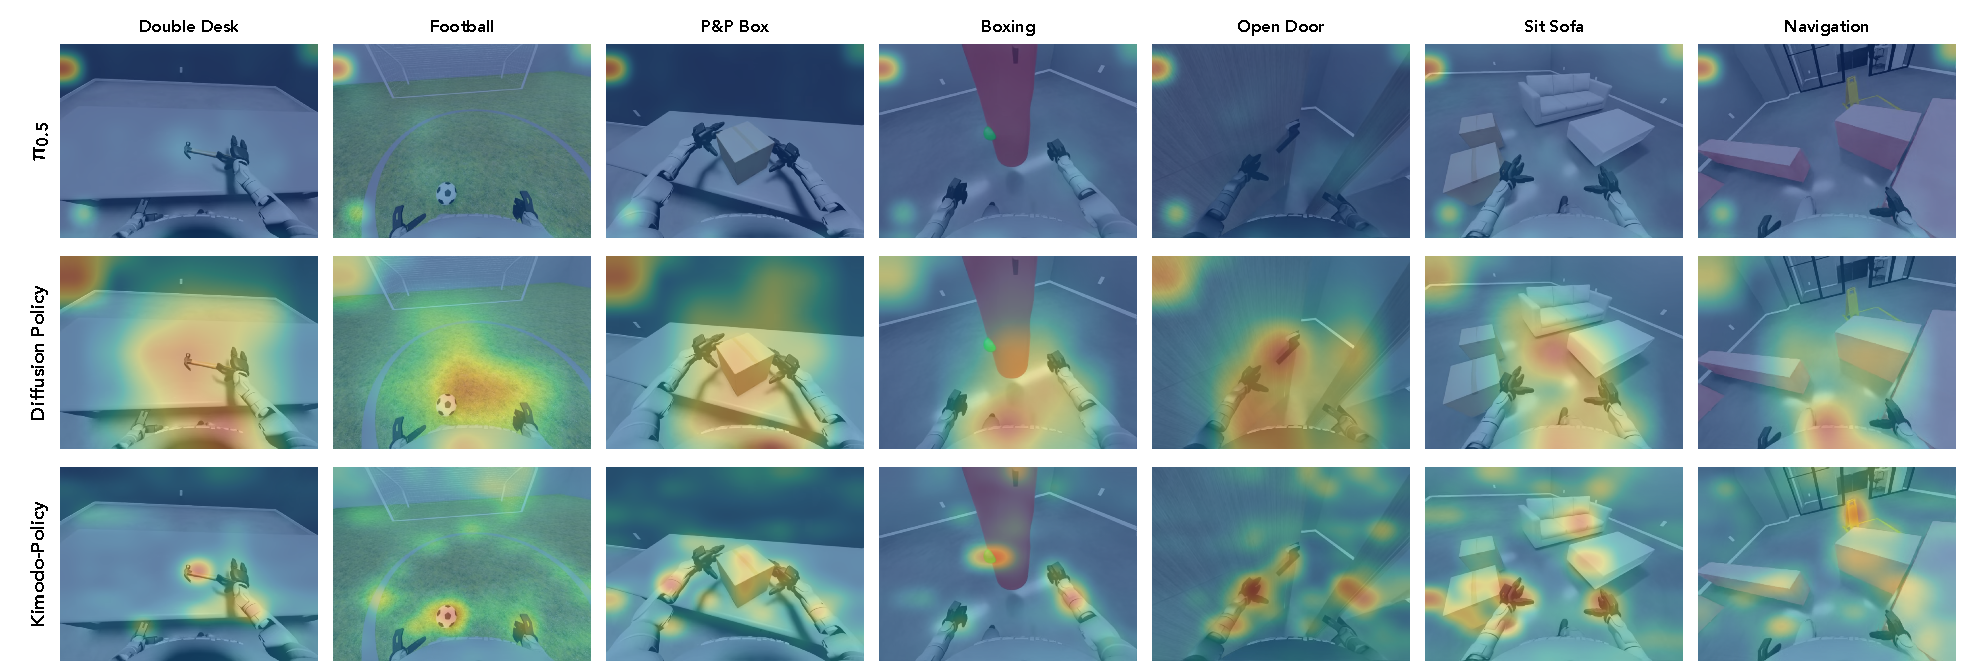
\includegraphics[width=\textwidth]{image/attention.pdf}
  \caption{\textbf{Task-Conditioned Visual Attention.} Qualitative attention maps for seven HumanoidArena tasks (columns: Double Desk, Football, P\&P Box, Boxing, Open Door, Sit Sofa, and Navigation); rows show $\pi_{0.5}$, Diffusion Policy, and Kimodo-Policy. Kimodo-Policy's attention shifts toward task-relevant objects and interaction regions across tasks.}
  \label{fig:attention}
\end{figure}

\subsection{Evaluation on the Simple Benchmark}
\label{sec:exp_simple}
We further evaluate Kimodo-Policy on the SIMPLE benchmark~\cite{simple}, using the L0--L2 protocol with progressively stronger visual, lighting, and target-pose randomization~\cite{simple}. We fine-tune an independent policy for each of the eight benchmark tasks and report the results in Table~\ref{table:simple_main_results}. This protocol isolates skill acquisition while testing robustness under increasing distribution shifts.

\begin{figure}[H]
  \centering
  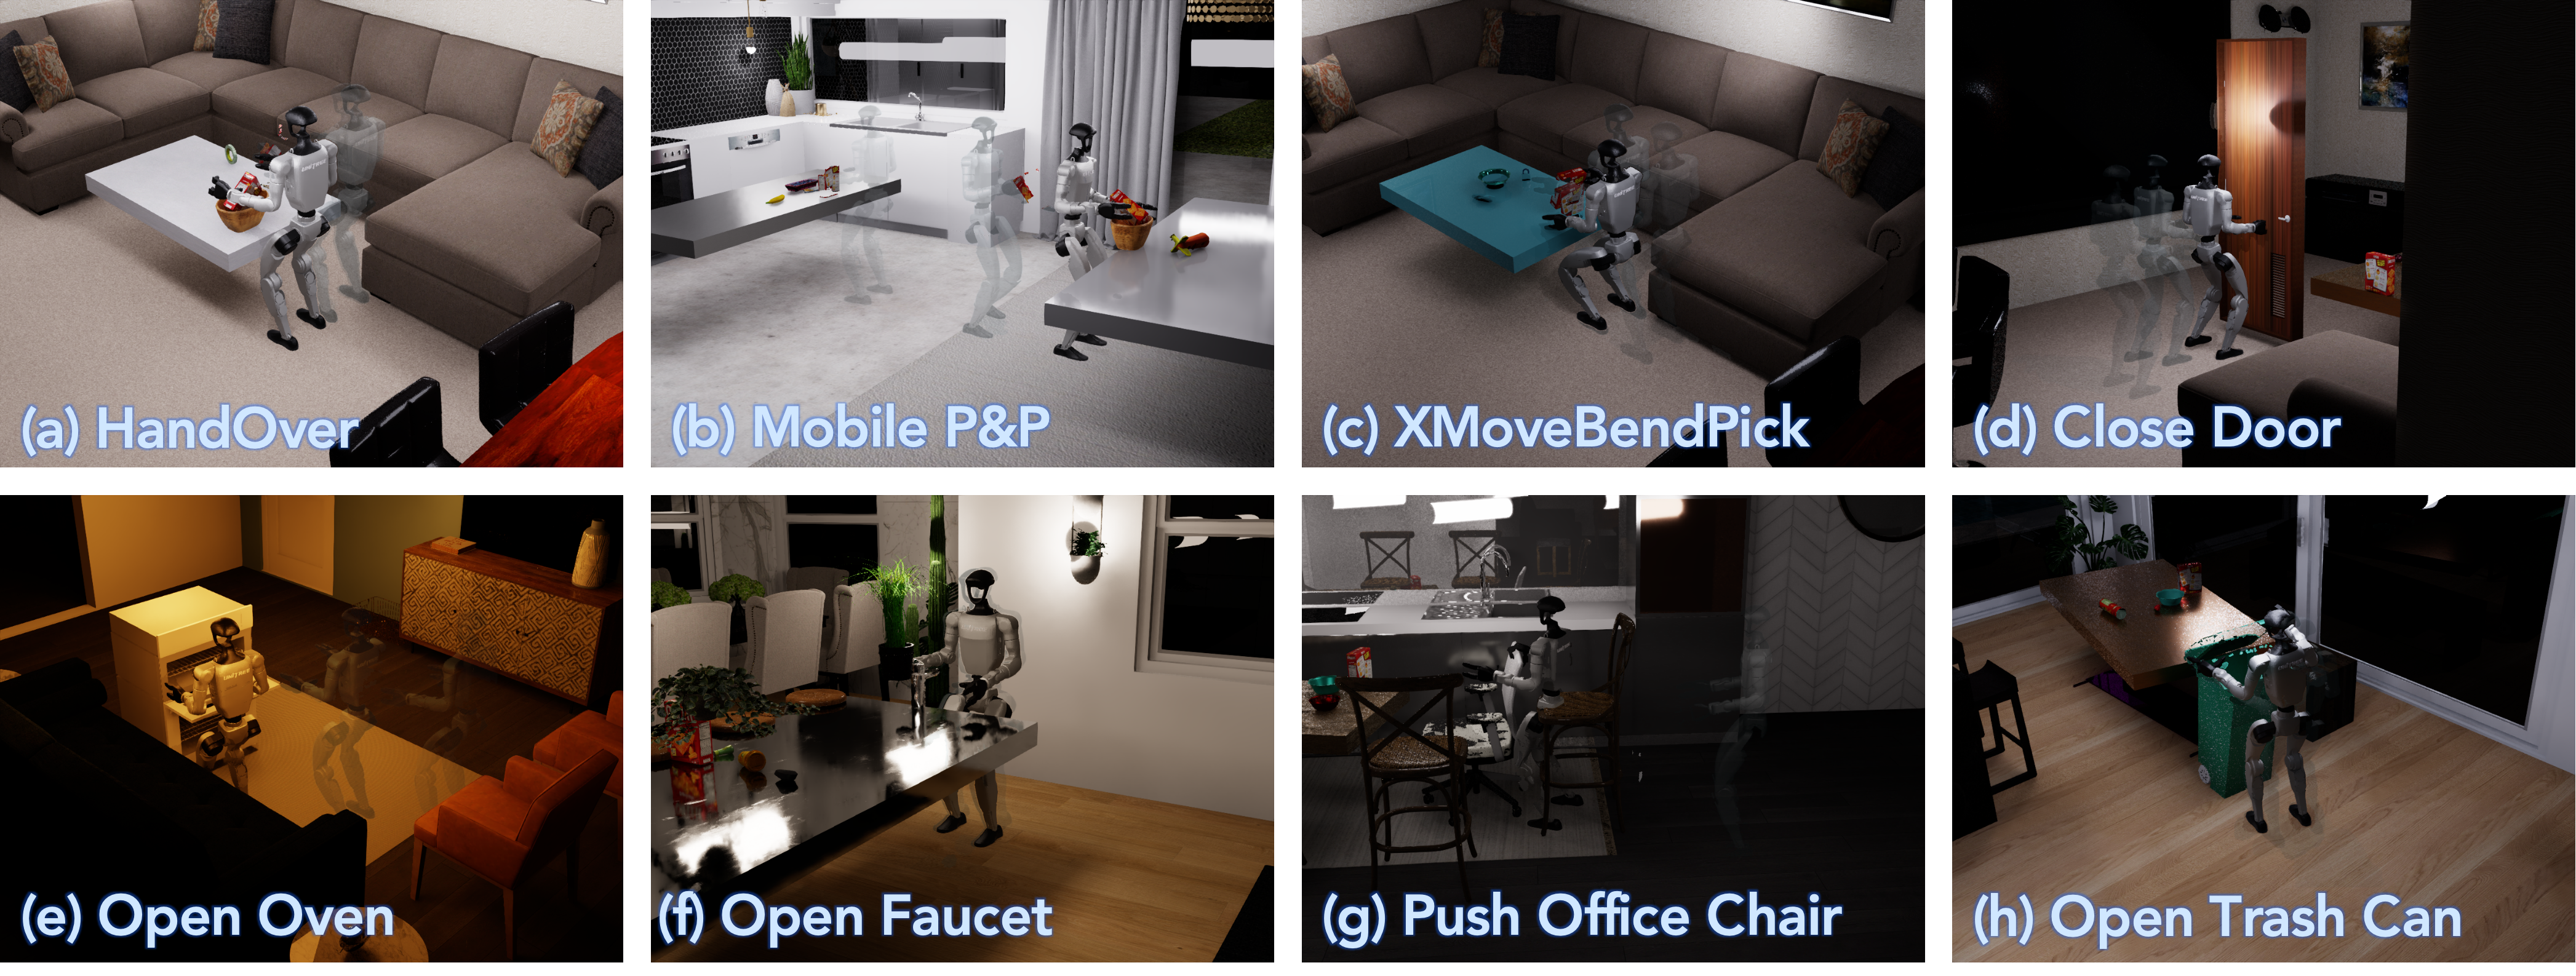
\includegraphics[width=\textwidth]{image/simple.png}
  \caption{\textbf{Evaluated SIMPLE Task Suite.} The selected tasks cover object handover and mobile pick-and-place, locomotion-integrated object pickup, articulated-object interaction, and household-object manipulation. Panels show (a) Handover, (b) Mobile P\&P, (c) XMoveBendPick, (d) CloseDoor, (e) OpenOven, (f) OpenFaucet, (g) Push Office Chair, and (h) OpenTrashCan.}
  \label{fig:simple_tasks}
\end{figure}

\textbf{Single-task results.} Table~\ref{table:simple_main_results} reports the VLA-pretrained Kimodo-Policy (\texttt{Ours}$^{*}$) on eight SIMPLE tasks, with success rates aggregated across the L0--L2 randomization levels. RTC is disabled to keep the evaluation comparable to the baselines. The policy attains the best or joint-best result on six tasks: it leads on Handover (83\% vs. 80\% for the strongest baseline), Mobile P\&P (70\% vs. 60\%), OpenOven (57\% vs. 53\%), and OpenFaucet (53\% vs. 33\%), and matches $\Psi_0$ at 100\% on CloseDoor and Push Office Chair. On the remaining tasks, it ranks second on XMoveBendPick (80\% vs. 93\% for $\Psi_0$) and OpenTrashCan (63\% vs. 83\%). This performance across handover, mobile manipulation, articulated-object interaction, and object pushing shows that Kimodo-Policy's motion-prior-based, visually grounded root--body--hand policy can support a broad range of humanoid manipulation skills under visual, lighting, and target-pose variation in the baseline-matched setting without RTC.

\begin{table}[H]
  \setlength{\belowcaptionskip}{6pt}
  \caption{\textbf{\textit{Single-Task Results on SIMPLE.}} L0--L2 progressively increase visual and lighting variation and target-pose randomization. Entries report L0/L1/L2 success counts and aggregate success rates (parentheses); bold/underlined values mark the best/second-best aggregate rates.}
  \label{table:simple_main_results}
  \centering
  \arrayrulecolor{hclblue}
  \setlength{\tabcolsep}{0pt}
  \renewcommand{\arraystretch}{1.08}
  \fontsize{6.2}{7}\selectfont
  \newcommand{\taskheader}[1]{{\fontsize{5.55}{6.2}\selectfont\textbf{\textsc{\hspace{2.2pt}#1\hspace{2.2pt}}}}}
  \newcommand{\resultentry}[2]{{\fontsize{5.2}{6}\selectfont\hspace{2.2pt}#1\;(#2)\hspace{2.2pt}}}
  \newcommand{\bestentry}[2]{{\fontsize{5.2}{6}\selectfont\textbf{\hspace{2.2pt}#1\;(#2)\hspace{2.2pt}}}}
  \newcommand{\secondentry}[2]{{\fontsize{5.2}{6}\selectfont\hspace{2.2pt}\underline{#1\;(#2)}\hspace{2.2pt}}}

  \begin{adjustbox}{width=\textwidth}
  \begin{tabular}{@{}c*{8}{c}@{}}
    \toprule
    {\fontsize{5.55}{6.2}\selectfont\textbf{Method}}
    & \taskheader{Handover}
    & \taskheader{Mobile P\&P}
    & \taskheader{XMoveBendPick}
    & \taskheader{CloseDoor}
    & \taskheader{OpenOven}
    & \taskheader{OpenFaucet}
    & \taskheader{Push Office Chair}
    & \taskheader{OpenTrashCan} \\
    \midrule

    $\Psi_0$~\cite{psi0}
    & \secondentry{7/7/10}{80\%}
    & \secondentry{7/5/6}{60\%}
    & \bestentry{10/9/9}{93\%}
    & \bestentry{10/10/10}{100\%}
    & \secondentry{7/5/4}{53\%}
    & \secondentry{3/3/4}{33\%}
    & \bestentry{10/10/10}{100\%}
    & \bestentry{7/9/9}{83\%} \\

    \rowcolor{hclbrown!15!white}
    \texttt{Ours}$^{*}$
    & \bestentry{9/8/8}{83\%}
    & \bestentry{9/8/4}{70.0\%}
    & \secondentry{10/7/7}{80\%}
    & \bestentry{10/10/10}{100\%}
    & \bestentry{8/4/5}{57\%}
    & \bestentry{5/6/5}{53\%}
    & \bestentry{10/10/10}{100\%}
    & \secondentry{9/4/6}{63\%} \\

    \bottomrule
  \end{tabular}
  \end{adjustbox}
\end{table}


\subsection{Evaluation on the Real-World Humanoid Robot}
\label{sec:exp_real}
We deploy Kimodo-Policy on a physical humanoid robot to assess language-conditioned loco-manipulation under unconstrained sensing and execution conditions. The evaluation covers eight tasks that require different combinations of locomotion, balance maintenance, single- and dual-arm coordination, and contact-rich manipulation. Figure~\ref{fig:real_world} shows Kimodo-Policy performing representative real-world tasks, illustrating how our method coordinates whole-body motion and manipulation during physical-robot execution. For each task, we execute ten trials and record the number of successful completions, providing a direct measure of deployment reliability across heterogeneous real-world interactions.

\begin{figure}[H]
  \centering
  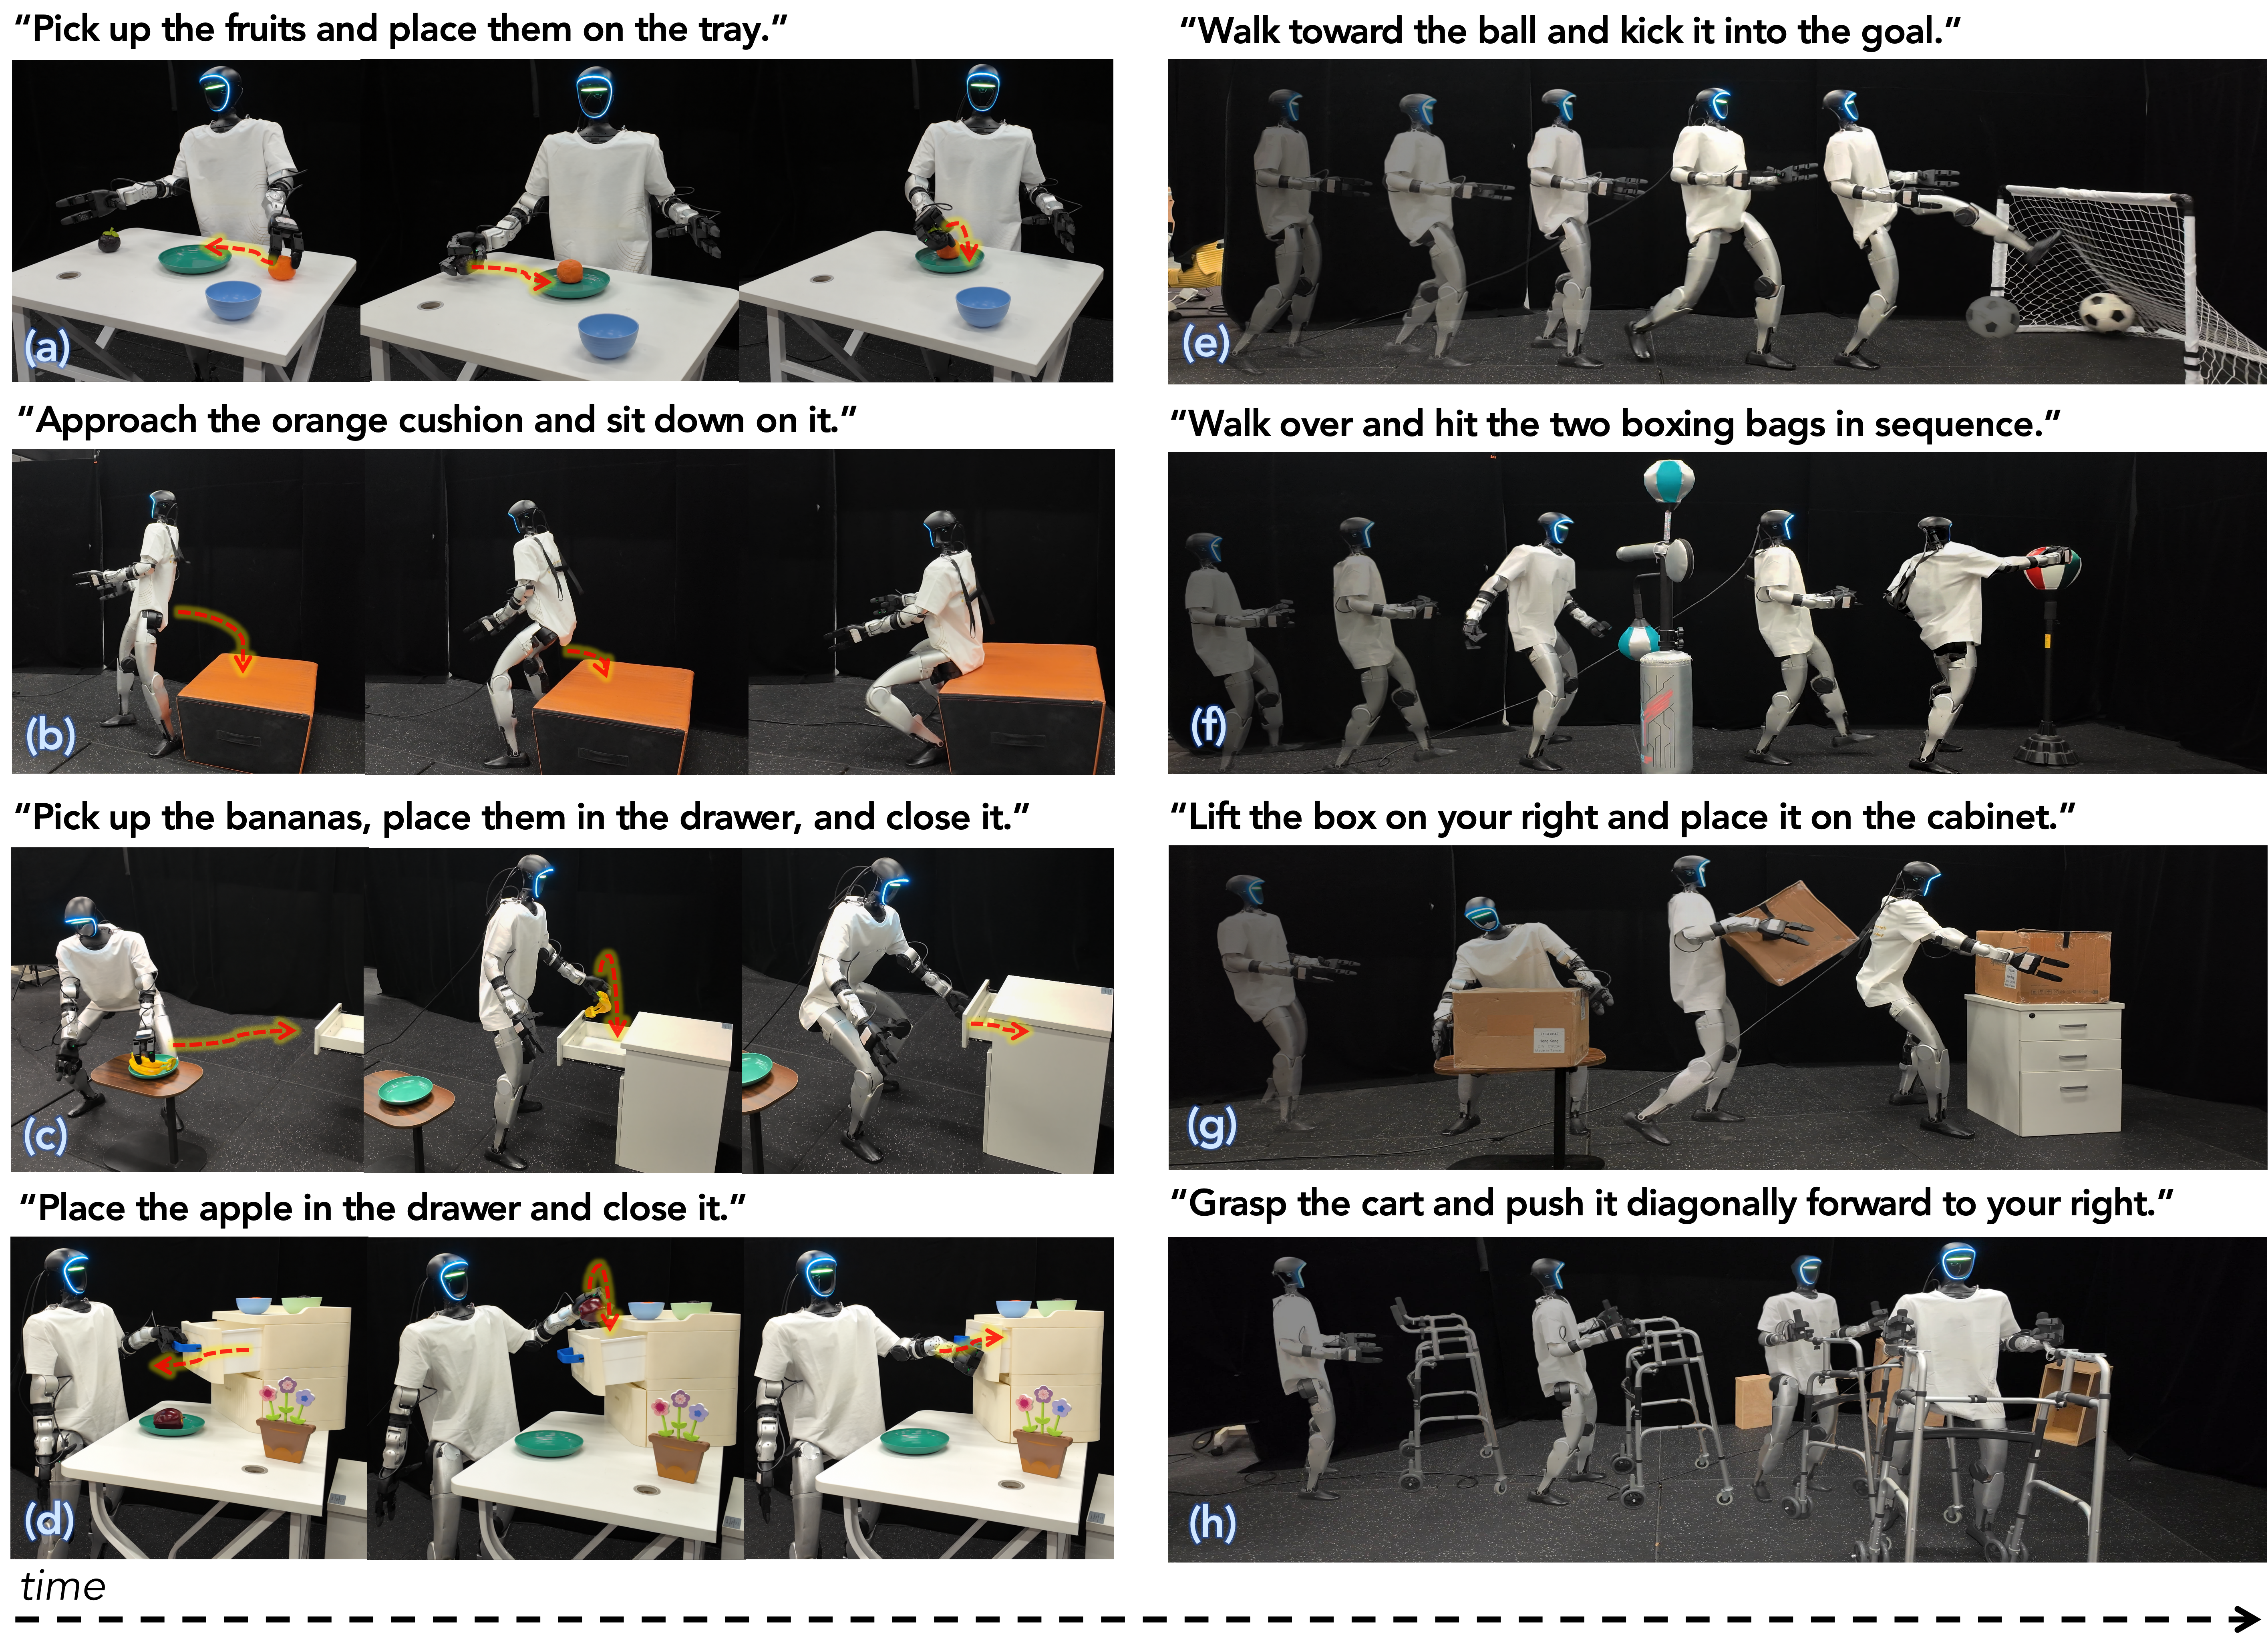
\includegraphics[width=\textwidth]{image/real_world.png}
  \caption{\textbf{Examples of Real-World Humanoid Manipulation.} The image shows representative interaction scenarios involving articulated objects, object transport, and coordinated whole-body motion.}
  \label{fig:real_world}
\end{figure}

\textbf{Real-world results.} Figure~\ref{fig:real_world_success_rates} compares task-level success across the eight physical-robot tasks. Kimodo-Policy trained from scratch achieves a mean success rate of 45\%, exceeding the reported averages of GR00T N1.6~\cite{grootn1} (31\%) and $\Psi_0$~\cite{psi0} (35\%). Initializing Kimodo-Policy with VLA-pretrained weights further raises the mean success rate to 60\%, a 15-percentage-point gain over the scratch-trained model. This gain is reflected across tasks: the pretrained policy improves success on seven tasks and matches the scratch model on Cart Pushing (60\%). Its strongest results are on Punching Bag (90\%), Cushion Sitting (80\%), and Dual-Arm PNP (70\%). Overall, the results indicate that VLA pretraining provides a useful initialization for adapting Kimodo-Policy to diverse real-world humanoid tasks, improving average performance while retaining competitive task-level success.

\begin{figure}[H]
  \centering
  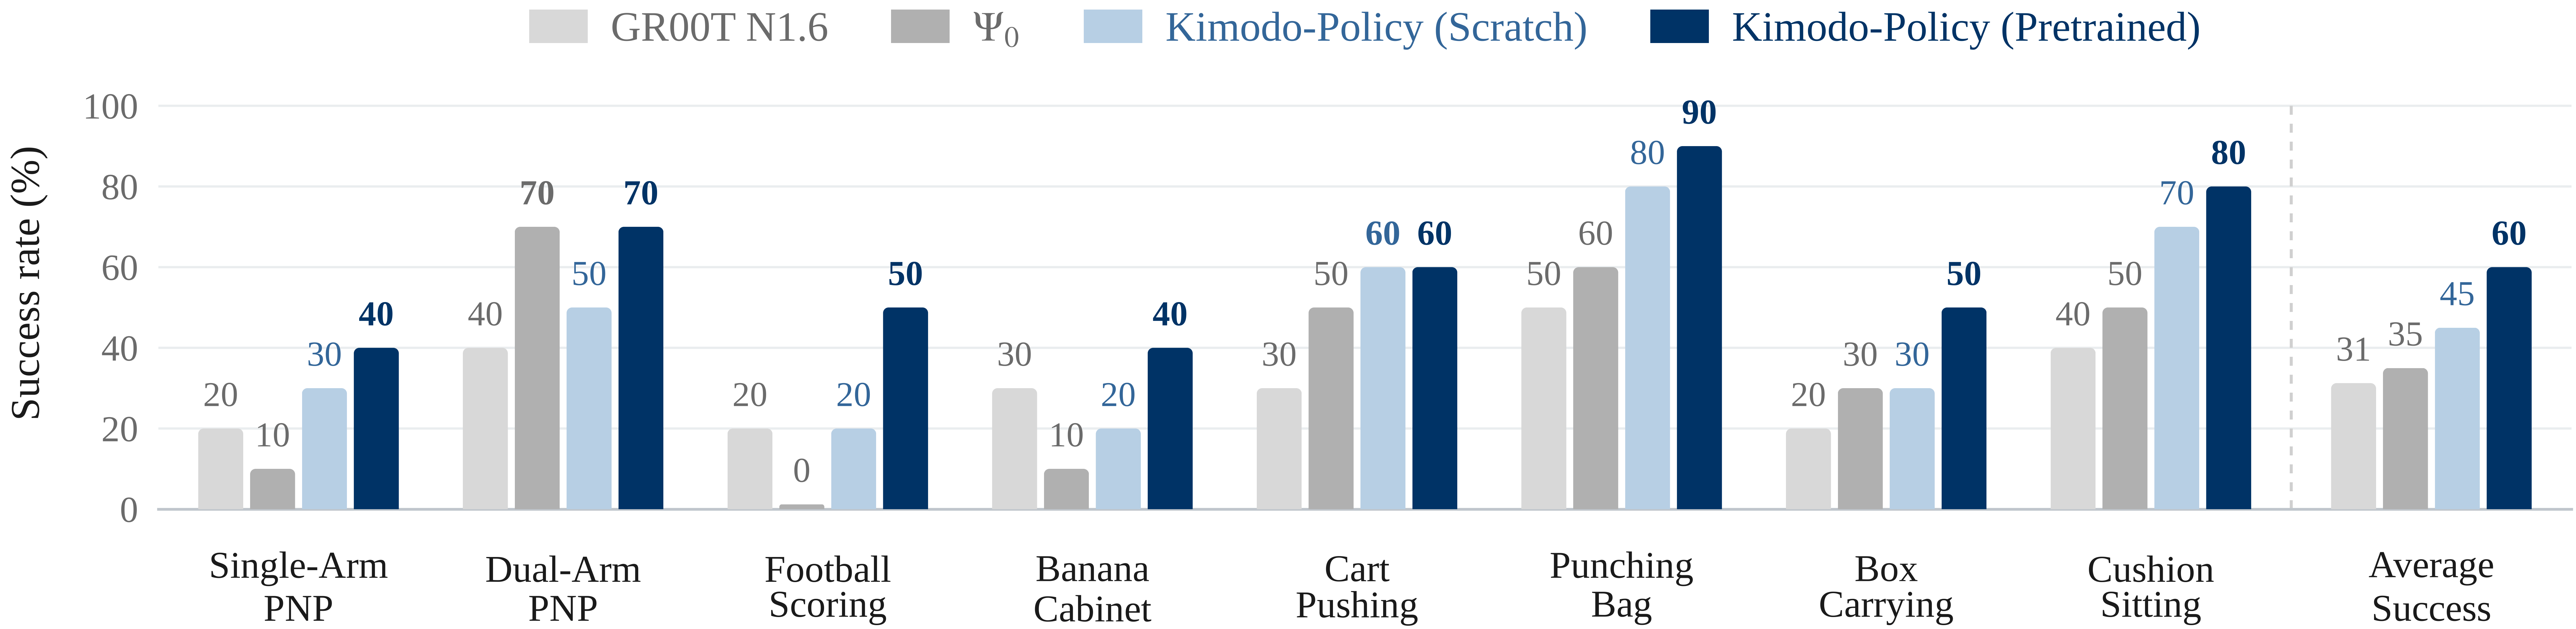
\includegraphics[width=\textwidth]{image/real_world_success_rates.png}
  \caption{\textbf{Real-World Success Rates Across Eight Tasks.} The plot compares GR00T N1.6, $\Psi_0$, and Kimodo-Policy trained from scratch or initialized with VLA pretraining. Bars report the success rate for each task; the rightmost group gives the mean across all eight tasks.}
  \label{fig:real_world_success_rates}
\end{figure}

\subsection{Does Better T2M Improve VLA Performance?}
\label{sec:exp_t2m}
Kimodo-Policy uses the pretrained Kimodo Text-to-Motion (T2M) model~\cite{kimodo} as its motion backbone, whose generated motions provide the structured prior for downstream whole-body control. This dependency raises a central question: does the quality of the motion prior directly affect the performance of the resulting VLA policy? To answer it, we compare two Kimodo-G1 variants within the same Kimodo-Policy architecture, adaptation procedure, and HumanoidArena protocol. Both variants contain 282M parameters; their motion corpora contain 288\,h and 700\,h for SEED-v1 and RP-v1, respectively, and both use a 90\%/10\% train/test split~\cite{kimodo}. This comparison examines how the choice of pretrained motion prior affects downstream VLA performance under a fixed policy architecture.
\begin{table}[H]
  \setlength{\belowcaptionskip}{6pt}
  \caption{
    \textbf{\textit{Effect of the T2M backbone on Kimodo-Policy.}} We compare two same-size Kimodo-G1 backbones using the same adaptation protocol. Data scales include the training and test splits; results are mean $\pm$ standard deviation over three seeds.}
  \label{tab:t2m_dependency}
  \centering
  \arrayrulecolor{hclblue}
  \begin{adjustbox}{max width=\textwidth}
  \setlength{\tabcolsep}{3.8pt}
  \renewcommand{\arraystretch}{1.08}

  \begin{tabular}{cccccc|ccccc}
  \toprule
  \multirow{2}{*}{\textbf{Base Model}} &
  \multirow{2}{*}{\textbf{Model Size}} &
  \multirow{2}{*}{\textbf{Data Scale}} &
  \multicolumn{3}{c|}{\textbf{Human--Object Interaction}} &
  \multicolumn{4}{c}{\textbf{Human--Scene Interaction}} &
  \multirow{2}{*}{\textbf{Overall~($\uparrow$)}} \\
  \cmidrule(lr){4-6}
  \cmidrule(lr){7-10}

  & & &
  \textbf{\textsc{Football}} &
  \textbf{\textsc{DoubleDesk}} &
  \textbf{\textsc{P\&Pbox}} &
  \textbf{\textsc{OpenDoor}} &
  \textbf{\textsc{SitSofa}} &
  \textbf{\textsc{Boxing}} &
  \textbf{\textsc{VisNavi}} \\
  \midrule

  \texttt{Kimodo-G1-SEED-v1}
  & 282\,M
  & 288\,h
  & \textbf{50.00$\pm$16.33\%}
  & \underline{33.33$\pm$15.46\%}
  & \underline{75.00$\pm$10.80\%}
  & \underline{60.00$\pm$4.08\%}
  & \underline{90.00$\pm$4.08\%}
  & \textbf{71.67$\pm$8.50\%}
  & \textbf{70.00$\pm$18.71\%}
  & \underline{64.29\%} \\

  \rowcolor{hclbrown!8!white}
  \texttt{Kimodo-G1-RP-v1}
  & 282\,M
  & 700\,h
  & \underline{35.0$\pm$7.1\%}
  & \textbf{40.0$\pm$0.0\%}
  & \textbf{80.0$\pm$4.1\%}
  & \textbf{93.3$\pm$6.2\%}
  & \textbf{96.7$\pm$4.7\%}
  & \underline{66.7$\pm$4.7\%}
  & \underline{61.7$\pm$6.2\%}
  & \textbf{67.63\%} \\

  \bottomrule
  \end{tabular}
  \end{adjustbox}
\end{table}

\textbf{T2M transfer results.} Table~\ref{tab:t2m_dependency} shows a task-dependent effect of the stronger T2M backbone. Kimodo-G1-SEED-v1, which uses the smaller BONES-SEED corpus, achieves an overall success rate of 64.29\%, whereas Kimodo-G1-RP-v1, which uses the 700\,h Rigplay corpus with the same parameter budget, reaches 67.63\%, corresponding to a 3.34-point improvement. The stronger backbone improves DoubleDesk from 33.33\% to 40.0\%, P\&Pbox from 75.0\% to 80.0\%, OpenDoor from 60.0\% to 93.3\%, and SitSofa from 90.0\% to 96.7\%. Football, Boxing, and VisNavi are lower for RP-v1, changing from 50.0\% to 35.0\%, 71.67\% to 66.7\%, and 70.0\% to 61.7\%, respectively. The aggregate improvement is therefore concentrated in the human--scene interaction tasks, while individual task performance remains sensitive to the pretrained motion prior. Since the policy architecture and training protocol are fixed, these results indicate that T2M capability can improve downstream VLA control.

\subsection{Does Performance Scale with Data and Model Size?}
\label{sec:exp_scaling}
To characterize how Kimodo-Policy responds to additional supervision and policy capacity, we conduct two controlled scaling sweeps. In the data sweep, we vary the duration of VLA policy-pretraining data while keeping the policy architecture, SonicX7 adaptation protocol, and evaluation setting fixed. In the model sweep, we vary the number of active policy parameters while using the same pretrained Text-to-Motion backbone, downstream data, optimization protocol, and evaluation suite. RTC is disabled throughout these evaluations to maintain the baseline-matched protocol used in the benchmark comparisons. This design isolates the effects of training data and model capacity on the downstream whole-body control performance of the proposed framework.

\begin{figure}[H]
  \centering
  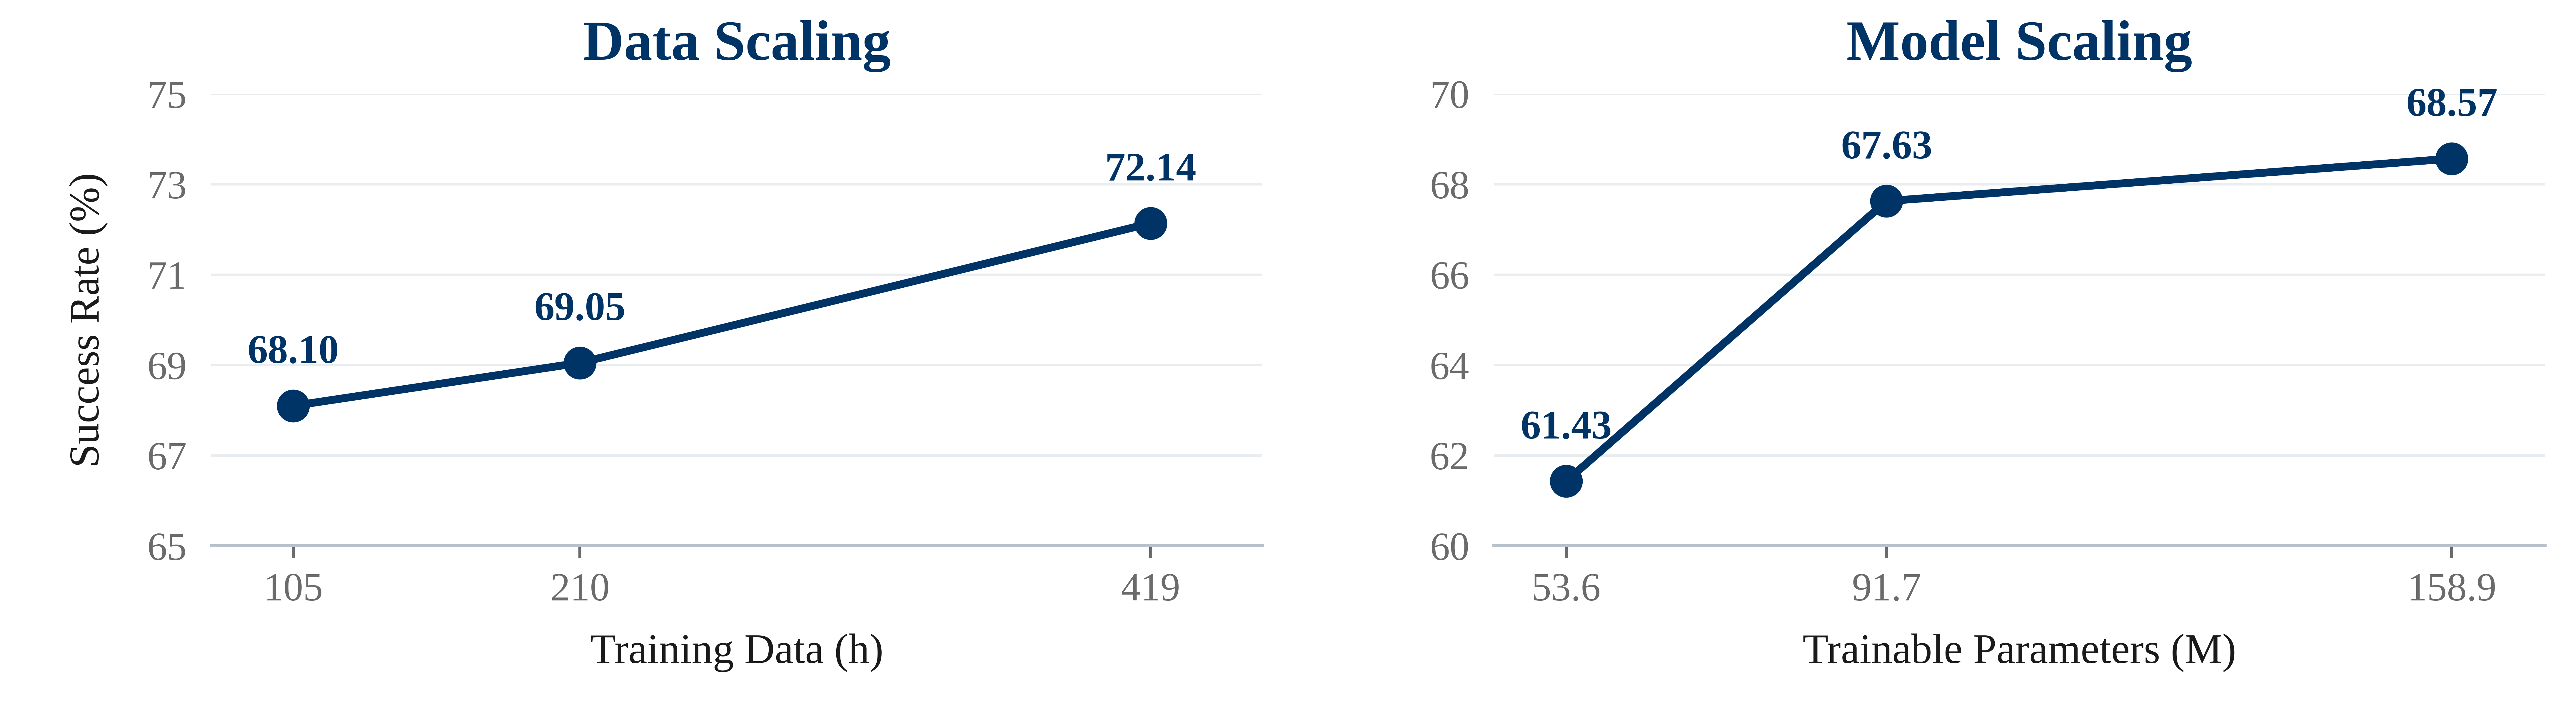
\includegraphics[width=\textwidth]{image/scaling_analysis.png}
  \caption{Scaling behavior of Kimodo-Policy. Left: overall success rate as a function of VLA policy-pretraining data duration. Right: overall success rate as a function of active policy parameters.}
  \label{fig:scaling_analysis}
\end{figure}

\textbf{Data scaling results.} Figure~\ref{fig:scaling_analysis} shows a consistent improvement as VLA policy-pretraining data increases: the overall success rate rises from 68.10\% with 105\,h to 69.05\% with 210\,h and 72.14\% with 419\,h, for a total gain of 4.04 percentage points. With the architecture, adaptation procedure, and evaluation protocol fixed, this trend demonstrates that Kimodo-Policy can translate additional humanoid demonstrations into stronger downstream control. In the proposed T2M-based framework, the pretrained motion prior supplies a structured basis for whole-body behavior, while broader VLA supervision improves how effectively visual observations and language instructions ground coordinated root, body, and hand actions. The consistent gains across the evaluated data scales point to further potential as larger and more diverse humanoid datasets become available.

\textbf{Model scaling results.} With the training data and optimization protocol held fixed, increasing active policy capacity yields higher overall success at every evaluated scale. The success rate improves from 61.43\% with 53.6M active parameters to 67.63\% with 91.7M, and reaches 68.57\% with 158.9M, for a 7.14-percentage-point gain from the smallest to the largest model. This improvement shows that additional capacity helps Kimodo-Policy represent multimodal conditioning and coordinate root, body, and hand predictions around its structured motion prior. The positive trend across all three configurations demonstrates that the proposed visually grounded, root--body--hand framework can benefit from increased capacity and motivates scaling to larger policies in conjunction with expanded training data.

\begingroup
% Use the official ICLR subsection formatting.
\subsection{Ablation Study}
\label{sec:exp_ablation}
\color{black}
We analyze the contribution of the pretrained T2M backbone, backbone freezing, VLA pretraining, the motion loss, and root--body gradient decoupling. All ablation variants are trained on a mixture of HumanoidArena tasks in the SONIC X7 setup and evaluated on DoubleDesk, Football, and P\&Pbox. Figure~\ref{fig:training_loss_comparison} shows the training-loss trajectories and the mean success rate across these three tasks for the corresponding model variants.
\begin{figure}[H]
  \centering
  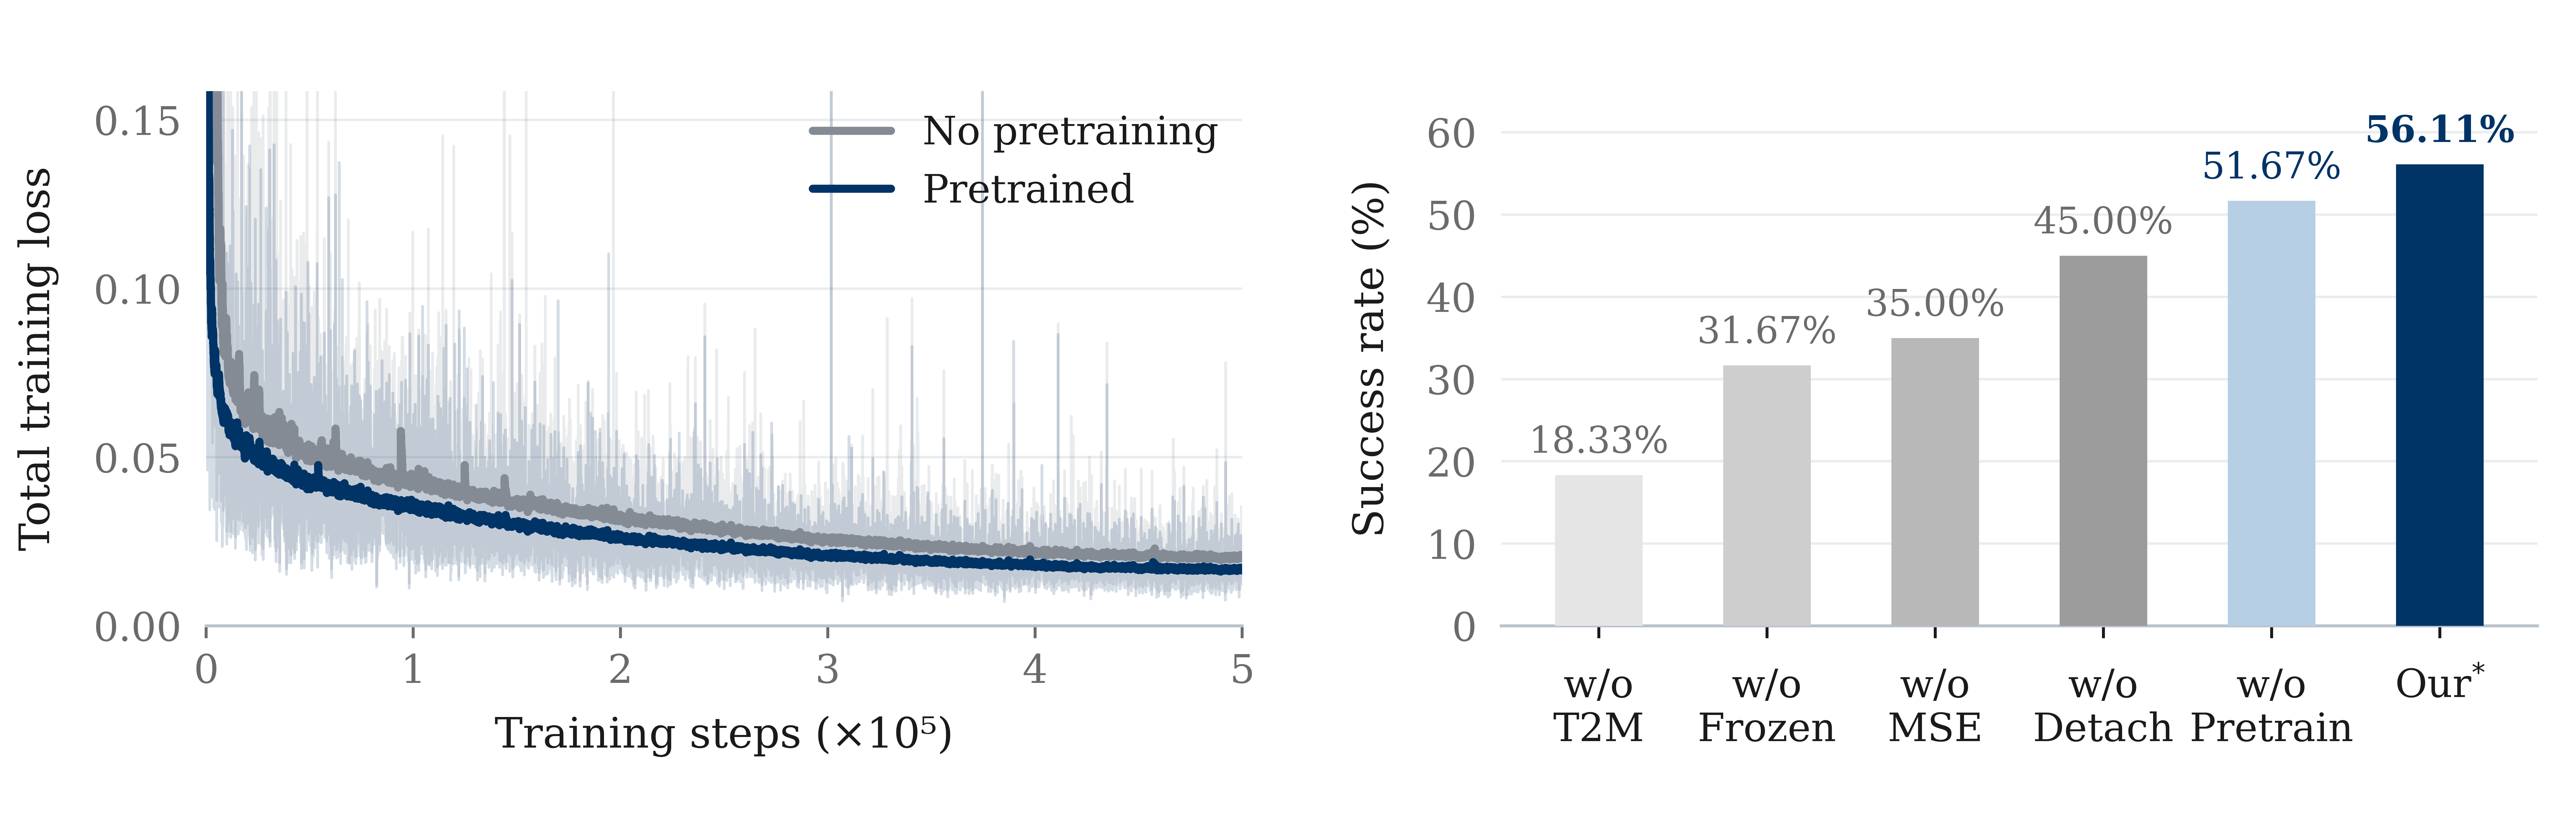
\includegraphics[width=\textwidth]{image/training_loss_comparison.png}
  \caption{\textbf{Training Dynamics and Ablation Performance.} Left: training-loss trajectories for the trained and no-training settings. Right: mean task success across DoubleDesk, Football, and P\&Pbox. Gray bars show component and training-design ablations: removing the T2M backbone (w/o T2M), unfreezing it (w/o Frozen), replacing MSE with the original Kimodo motion loss (w/o MSE), and removing root--body gradient detachment (w/o Detach). The VLA-pretraining comparison is shown separately in light blue (w/o Pretrain) and dark blue (Ours$^{*}$).}
  \label{fig:training_loss_comparison}
\end{figure}



\textbf{Effect of the pretrained motion prior and backbone freezing.} Without VLA pretraining, Kimodo-Policy achieves 51.67\% mean success. Removing the pretrained T2M backbone reduces success to 18.33\%, demonstrating the substantial contribution of the motion prior to downstream whole-body control. Unfreezing the backbone also degrades performance to 31.67\%, supporting the preservation of pretrained motion representations during policy adaptation. Together, these results validate our strategy of retaining a frozen motion generator while learning visual and task conditioning through dedicated trainable branches, enabling effective control without additional VLA pretraining.

\textbf{Effect of the prediction objective and root--body gradient decoupling.} Under the same setting without VLA pretraining, replacing MSE with the original Kimodo motion objective reduces success from 51.67\% to 35.00\%. This supports combining a preserved motion prior with direct supervision of policy prediction targets for downstream adaptation. Removing root--body gradient detachment further reduces success to 45.00\%. Detachment retains root-to-body conditioning while preventing the body loss from updating the root ControlNet, allowing each stage to learn through its own objective while preserving coordinated generation. These findings support direct prediction supervision and controlled cross-stage gradient flow as effective choices for adapting the structured motion prior to policy learning.

\textbf{Effect of VLA pretraining.} VLA pretraining further improves success from 51.67\% to 56.11\%, accompanied by generally lower training loss and smaller fluctuations. Since both variants retain the pretrained T2M backbone, this gain reflects the complementary benefit of learning visual and task conditioning beyond the motion prior itself. Collectively, the results support Kimodo-Policy's central design: preserving pretrained motion-generation capabilities, adapting them through dedicated conditioning branches and stage-specific optimization, and strengthening visually grounded control through VLA pretraining.


\endgroup
